\chapter{Digital Meets the Analog World: DAC, ADC, PWM}
\label{ch:analog}

In the previous chapter we saw that a chip pin delivers current and that ``0'' and ``1'' are
voltage ranges. One question remains: what do we do when we need something that is \emph{neither} 0 nor
1? A buzzer must sound at the right pitch, an LED must glow at half brightness, and a
temperature sensor outputs a voltage that has to be turned into a number. This
chapter covers two bridges between the digital and the continuous world.

\begin{buildbox}
The \emph{Learn} tab, the ``Circuits and the board'' book, the ``Connecting to the board'' chapter, the lesson
``A buzzer''. Put a buzzer on the Lab bench and connect its S input to the
board. Read in the lesson how an active buzzer differs from a passive one:
what signal must you apply to a passive one to make it sound? Write down the
answer---you will need it in the section on PWM.
\end{buildbox}

Everything we have studied so far lives in a discrete world: signals take
the values 0 or 1, and time advances in clock cycles. But the world around us is continuous. A temperature
sensor outputs a voltage, a microphone outputs an alternating current, and a loudspeaker
needs a continuous oscillation. On the boundary between digital and analog
technology stand two kinds of devices: an \term{ADC} (analog-to-digital converter)
turns a voltage into a number, and a \term{DAC} (digital-to-analog converter)
turns a number into a voltage.

\section{Sampling and Quantization}

Converting an analog signal into a digital one takes two steps. First the
voltage is measured at equal intervals of time---this is
\term{sampling}, and the measurement rate is called the \term{sampling
rate}. Then each measurement is rounded to the nearest of
$2^N$ levels---this is \term{quantization}, and $N$ is the resolution of the converter in bits.

\begin{figure}[H]
\centering
\begin{tikzpicture}[x=1.15cm,y=1.5cm, font=\sffamily\scriptsize]
  \draw[->] (-0.1,0) -- (7.0,0) node[right] {time};
  \draw[->] (0,-1.3) -- (0,1.4) node[above] {$U$};
  \foreach \l in {-1,-0.667,-0.333,0,0.333,0.667,1} \draw[gray!40] (0,\l) -- (6.6,\l);
  \draw[FpgaBlue, thick, domain=0:6.28, samples=120, smooth] plot (\x, {sin(\x r)});
  \foreach \i in {0,...,12} {
    \pgfmathsetmacro{\v}{sin(\i*0.5 r)}
    \pgfmathsetmacro{\q}{round(3*\v)/3}
    \draw[FpgaOrange] (\i*0.5,0) -- (\i*0.5,\q);
    \fill[FpgaOrange] (\i*0.5,\q) circle (1.6pt);
  }
  \node[FpgaBlue, anchor=west] at (4.3,1.15) {continuous signal};
  \node[FpgaOrange!80!black, anchor=west] at (4.3,0.85) {samples after quantization};
\end{tikzpicture}
\caption{Sampling (samples every $0.5$~s) and quantization (7 levels). The orange values are closest to the blue curve but do not coincide with it}
\end{figure}

Quality depends on the sampling rate and the resolution. The
Nyquist--Shannon sampling theorem states that a signal with the highest frequency
$f_{max}$ can be reconstructed without loss if it is measured at a rate
of at least $2 f_{max}$. That is why for sound up to 20~kHz compact discs use
44.1~kHz. The resolution determines the quantization step: for a reference voltage
$U_{\text{ref}}$ and a resolution of $N$ bits, one \term{least significant bit} (LSB) corresponds to
\[
U_{LSB} = \frac{U_{\text{ref}}}{2^N}.
\]
For 8 bits and 3.3~V we get $3.3/256 \approx 12.9$~mV. Each
additional bit doubles the number of levels and adds about 6~dB to the
quantization signal-to-noise ratio.

\begin{diybox}[Samples and Resolution]
\textbf{Task.} See how a table of samples produces a periodic signal, and
estimate the effect of resolution.\\
\textbf{In Logra.} The \emph{Examples} tab: \code{lookup-sine} and
\code{dds-tone}; the \emph{Waveforms} tab.\\
\stars{1} \emph{Repeat.} In \code{lookup-sine} shorten the step and follow in the
waveform a full period of the sample table: how many samples fall in one
period?\\
\stars{2} \emph{Modify.} Change one sample of the table and find in the waveform the
clock cycle at which the shape of the signal changed.\\
\stars{3} \emph{Project.} In \code{dds-tone} set the tuning word to
$16384$, follow the four phases over a period, and compute the signal frequency from
the formula $f = f_\text{clk}\cdot F/65536$ (no speaker connected).\\
\textbf{Expected result.} The word $16384$ gives four samples per period:
the frequency is a quarter of the clock frequency.\\
\textbf{How to check.} The \emph{Waveforms} tab: the period of the digital signal
is four clock cycles.
\end{diybox}

\section{The DAC: From a Number to a Voltage}

The most illustrative DAC is the \term{$R$--$2R$ resistor ladder}. A binary
code controls the switches, each bit contributes to the output voltage
half as much as the previous one, and the output is a value proportional to the
code.

\begin{figure}[H]
\centering
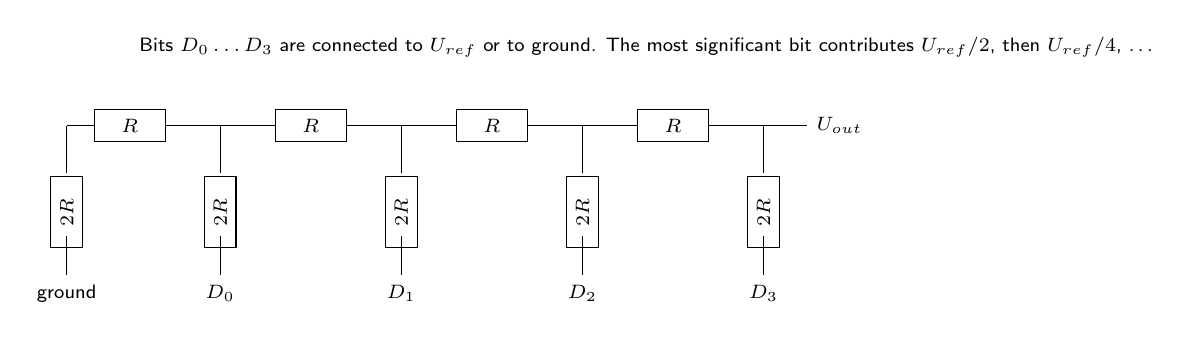
\begin{tikzpicture}[font=\sffamily\scriptsize, res/.style={draw, minimum width=9mm, minimum height=3.6mm, fill=white}]
  \draw (-0.8,0) -- (8.6,0) node[right] {$U_{\text{out}}$};
  \foreach \i in {0,1,2,3} {
    \pgfmathsetmacro{\x}{\i*2.3+1.15}
    \node[res] at (\i*2.3,0) {$R$};
    \draw (\x,0) -- (\x,-0.6);
    \node[res, rotate=90] at (\x,-1.1) {$2R$};
    \draw (\x,-1.4) -- (\x,-1.9) node[below] {$D_{\i}$};
  }
  \draw (-0.8,0) -- (-0.8,-0.6);
  \node[res, rotate=90] at (-0.8,-1.1) {$2R$};
  \draw (-0.8,-1.4) -- (-0.8,-1.9) node[below] {ground};
  \node[align=left, anchor=west] at (0,1.0) {Bits $D_0\ldots D_3$ are connected to $U_{\text{ref}}$ or to ground. The most significant bit contributes $U_{\text{ref}}/2$, then $U_{\text{ref}}/4$, \ldots};
\end{tikzpicture}
\caption{The $R$--$2R$ ladder (simplified): each bit controls a switch between $U_{\text{ref}}$ and ground}
\end{figure}

A digital chip usually has no ready-made DAC, but the easiest way to get one is
from ordinary digital blocks. Instead of resistors we use
\term{pulse-width modulation} (PWM): the output switches quickly between 0
and 1, and the fraction of the period that it is high (the duty cycle) is proportional to the required
value. A simple $RC$ filter averages these pulses and turns them into a
constant voltage. An LED driven by PWM ``breathes'' because the eye
averages the pulses in exactly the same way as the filter.

A PWM circuit consists of two parts: an eight-bit counter that
cyclically counts from 0 to 255, and a comparator that compares the counter with the
required value \code{level}. While the counter is less than \code{level}, the output is
one, otherwise zero. If, for example, \code{level} is 64, then the one is held for
64 clock cycles out of 256, so the average voltage is $64/256 = 25\,\%$ of
the supply.

\begin{figure}[H]
\centering
\begin{tikzpicture}[x=1.0cm, y=0.9cm, font=\sffamily\small]
  % counter: two periods of the sawtooth
  \draw[->] (-0.2,0) -- (9.2,0) node[right] {$t$};
  \draw[->] (0,-0.2) -- (0,4.4) node[above] {counter};
  \draw[FpgaBlue, very thick] (0,0) -- (4,4) -- (4,0) -- (8,4) -- (8,0);
  \draw[FpgaOrange, thick, dashed] (0,1) -- (9,1) node[right] {\code{level}};
  \node[anchor=east] at (0,4) {255};
  \node[anchor=east] at (0,1) {64};
  % output
  \begin{scope}[yshift=-3.2cm]
    \draw[->] (-0.2,0) -- (9.2,0) node[right] {$t$};
    \draw[FpgaGreen!60!black, very thick] (0,0) -- (0,1) -- (1,1) -- (1,0) -- (4,0) -- (4,1) -- (5,1) -- (5,0) -- (8,0) -- (8,1) -- (9,1);
    \node[anchor=east] at (0,0.5) {pwm};
    \draw[<->] (0,-0.5) -- node[below] {1 period = 256 clock cycles} (4,-0.5);
    \draw[<->] (0,1.5) -- node[above] {64 clock cycles} (1,1.5);
  \end{scope}
\end{tikzpicture}
\caption{PWM: the output is one while the counter sawtooth is below the \code{level}}
\label{fig:pwm_wave}
\end{figure}

The PWM frequency is $f_{\text{clk}}/256$: at 27~MHz this is about 105~kHz, and
a simple $RC$ filter with a time constant of tens of microseconds is enough for
smoothing. The drawback of the method is its slow response: a new value
needs at least one period.

\subsection{Sound: A Buzzer on PWM}

A passive buzzer reproduces the frequency that is applied to it. So for
sound we need not a level but a \emph{periodic signal}: rectangular
pulses at the tone frequency. To get, for example, a 2~kHz tone from a 27~MHz
clock, the output must toggle every $27\,000\,000/(2\cdot 2000)
= 6750$ clock cycles. The duty cycle sets the loudness: at 50\,\% the sound is loudest, and with a
small fraction of one it is quieter.

\begin{diybox}[Project Stage 10: A PWM Buzzer]
\textbf{Task.} Add an alarm sound to the panel and connect it to the
board.\\
\textbf{In Logra.} The \emph{Learn} tab: the lesson ``A buzzer'' (the chapter ``Connecting to the
board'') and the lesson ``A button on a real board''; the \emph{Examples} tab: \code{pwm},
\code{breathing-pwm}; the \emph{Waveforms}, \emph{Pins}, and \emph{Connect} tabs.\\
\stars{1} \emph{Repeat.} The lesson ``A buzzer'': put the buzzer on the bench and connect
its S input to the board. In the \code{pwm} example follow how the level sets the fraction of
one.\\
\stars{2} \emph{Modify.} Problem~4: apply the code 192 and measure the duty cycle in
\emph{Waveforms} (expected 75\,\%). Then in \code{breathing-pwm} shorten
\code{LEVEL\_TICKS} and find the turning points of the level at the bounds 0 and 255.\\
\stars{3} \emph{Project.} \textbf{A stage of the ``Security Panel'' project:} the PWM
buzzer. The ALARM state (stage~9) switches on a 2~kHz tone with a duty cycle of 25\,\%;
outside of the alarm the buzzer output is zero. Acceptance criterion: in the waveform the
tone period is 13\,500 clock cycles at a 27~MHz clock frequency, the fraction of one
in the period is 25\,\%, and when the alarm ends the sound stops on the
next clock cycle. Then connect the buzzer in the \emph{Connect} tab
(assign a port in the \emph{Pins} tab), program the board, and check that the tone
is audible.\\
\textbf{Expected result.} The buzzer sounds exactly in the ALARM state and
is silent in the others.\\
\textbf{How to check.} The \emph{Waveforms} tab: the buzzer output and the panel state
on one time scale; the \emph{Pins} tab: the buzzer port is assigned.
\end{diybox}

\section{The ADC: From a Voltage to a Number}

There are several ways to build an ADC, and each has its own price.

\begin{table}[H]
\centering
\caption{Main types of ADC}
\small
\begin{tabularx}{\textwidth}{l X X}
\toprule
\textbf{Type} & \textbf{How it works} & \textbf{Feature} \\
\midrule
Parallel (flash) & $2^N-1$ comparators compare the input with a ladder of voltages simultaneously & Instantaneous, but huge: 8 bits need 255 comparators \\
Successive approximation (SAR) & $N$ clock cycles of a bisection search with one comparator and a DAC & The golden mean: fast and cheap, the most widespread \\
Sigma-delta & A one-bit ADC at a very high rate with a digital filter & Very accurate, but slow; used in audio and measuring instruments \\
Integrating & Measures the discharge time of a capacitor & Very accurate, but slow; multimeters \\
\bottomrule
\end{tabularx}
\end{table}

\subsection{The Successive-Approximation ADC}

The idea is similar to the game ``guess a number from 0 to 255'': each time we name the middle of
the remaining interval and, depending on the answer ``higher'' or ``lower'', discard half.
In $N$ questions we find the number to within one bit. The role of the
``question'' is played by a comparator, which compares the input voltage with the
DAC voltage, and the role of the host is played by a digital machine, which checks the bits one by one
from the most significant to the least significant.

\begin{figure}[H]
\centering
\begin{tikzpicture}[font=\sffamily\small, bx/.style={draw, minimum width=26mm, minimum height=11mm, fill=white, rounded corners=2pt, align=center}]
  \node[bx] (cmp) at (0,0) {Comparator};
  \node[bx, minimum width=36mm] (sar) at (5.2,0) {SAR machine\\{\scriptsize register + control}};
  \node[bx] (dac) at (5.2,-2.2) {DAC};
  \draw[-{Stealth}] (-2.6,0.25) node[left] {$U_{\text{in}}$} -- ([yshift=2.5mm]cmp.west);
  \draw[-{Stealth}] (dac.west) -| node[pos=0.25, above] {$U_{\text{DAC}}$} ([xshift=-4mm]cmp.south);
  \draw[-{Stealth}] (cmp) -- node[above] {cmp} (sar);
  \draw[-{Stealth}] (sar) -- node[right] {code} (dac);
  \draw[-{Stealth}] (sar.east) -- ++(1.4,0) node[right] {result};
\end{tikzpicture}
\caption{Structure of a successive-approximation ADC. The digital part is a finite-state machine, which means it is implemented entirely by a digital circuit}
\end{figure}

The digital part is a finite-state machine with a result register: from the signal
\code{cmp} it decides whether to keep the bit under test as one. Let us follow its operation for
an input voltage that corresponds to the number 179 ($\text{B3}_{16}=10110011_2$).

\begin{table}[H]
\centering
\caption{Searching for the number 179 by successive approximation}
\small
\begin{tabular}{clccl}
\toprule
\textbf{Step} & \textbf{Trial (DAC code)} & \textbf{In decimal} & \textbf{$U_{\text{in}}\ge U_{\text{DAC}}$?} & \textbf{Result after the step} \\
\midrule
1 & \code{0x80} = \code{10000000} & 128 & yes & \code{0x80} \\
2 & \code{0xC0} = \code{11000000} & 192 & no & \code{0x80} \\
3 & \code{0xA0} = \code{10100000} & 160 & yes & \code{0xA0} \\
4 & \code{0xB0} = \code{10110000} & 176 & yes & \code{0xB0} \\
5 & \code{0xB8} = \code{10111000} & 184 & no & \code{0xB0} \\
6 & \code{0xB4} = \code{10110100} & 180 & no & \code{0xB0} \\
7 & \code{0xB2} = \code{10110010} & 178 & yes & \code{0xB2} \\
8 & \code{0xB3} = \code{10110011} & 179 & yes & \code{0xB3} \\
\bottomrule
\end{tabular}
\end{table}

Eight steps give eight bits of the result: at each step the machine checks
exactly one bit, starting from the most significant. \lookahead{you will find a text implementation of this machine
and a waveform of its operation in Chapter~\ref{ch:bridge}.}

\begin{infobox}[An ADC and a Digital Chip]
Many digital chips have no ``slow'' ADC like the one in a microcontroller.
If you need to measure a voltage, you connect an external ADC chip over a
serial interface. \lookahead{on the board from Part~II this is exactly how it is done;
the interfaces are covered in Chapter~\ref{ch:uart}.}
\end{infobox}

\begin{diybox}[The ADC: Finding a Number Bit by Bit]
\textbf{Task.} Trace the operation of a successive-approximation ADC and
see that the result is produced by a digital machine, not by an analog circuit.\\
\textbf{In Logra.} The \emph{Examples} tab: \code{sigma-delta};
the \emph{Waveforms} and \emph{RTL} tabs.\\
\stars{1} \emph{Repeat.} Carry out by hand the search for the number 179 using the table in this chapter
and write out the trial DAC codes.\\
\stars{2} \emph{Modify.} Problem~6: write out the trial codes for the number 100 and
compare them with the sample answer.\\
\stars{3} \emph{Project.} In the \code{sigma-delta} example, after the level has settled,
count 64 clock cycles: level 16 gives 16 ones, level 48 gives 48.
Explain how the density of ones is similar to PWM and how it differs.\\
\textbf{Expected result.} The number of ones in 64 clock cycles equals the level.\\
\textbf{How to check.} The \emph{Waveforms} tab: count the ones in 64 clock cycles;
the \emph{RTL} tab: find the accumulator (the remainder register) and its carry.
\end{diybox}

\begin{warnbox}[Common mistakes]
\begin{itemize}
  \item \textbf{Confusing resolution and accuracy.} Many bits give a small step
        $U_\text{LSB}$, but do not remove the noise and the error of the reference voltage.
  \item \textbf{Taking the sampling rate exactly $2f_\text{max}$ with no margin.}
        Real signals are wider than ideal ones; the rate is chosen with a margin.
  \item \textbf{Applying PWM without a filter where a constant
        voltage is needed.} Without filtering you get not an ``average voltage'' but
        fast pulses.
  \item \textbf{Expecting an instant response from a PWM DAC.} A new value
        fully appears only after one period, so a slow PWM cannot be
        used for a fast signal.
\end{itemize}
\end{warnbox}

\section{Questions and Problems}
\label{sec:tasks-analog}

The answers are collected in Appendix~\ref{app:answers}.

\begin{taskbox}[Chapter Problems]
\begin{enumerate}
  \item \stars{1}~A 10-bit ADC with a reference voltage of 3.3~V. What voltage change
        corresponds to one least significant bit?
  \item \stars{1}~How many bits are needed to distinguish voltages with a step of at most
        10~mV in the range 0--5~V?
  \item \stars{1}~At what minimum rate must a signal with a frequency of
        up to 3~kHz be measured so that it can be reconstructed from the samples?
  \item \stars{1}~The code 192 is applied to the input of a PWM DAC. What fraction of the time is
        the output equal to one? What average voltage do you get at a supply of
        3.3~V?
  \item \stars{2}~How many conversion clock cycles does a 12-bit successive-approximation
        ADC need? How many comparators does a 12-bit parallel
        ADC need?
  \item \stars{2}~Describe which values a successive-approximation ADC will try
        when measuring the code 100 (eight bits).
  \item \stars{2}~\emph{Find the error.} In the search for the number 100 a student wrote:
        ``step 1: try \code{0x80}, answer no, result \code{0x80}; step 2:
        try \code{0xC0}\ldots''. What is wrong, and what trial
        code should be at the second step?
  \item \stars{3}~\emph{Mini-project.} Build an eight-bit PWM from a counter and a
        comparator. Acceptance criterion: in the waveform at \code{level}=64 the output
        is one for 64 clock cycles out of 256, at \code{level}=0 the output is zero all the time,
        and at \code{level}=255 it is one for 255 clock cycles out of 256.
  \item \stars{3}~\emph{Mini-project (stage~10).} The panel buzzer output: in the ALARM state
        it produces a 2~kHz tone with a duty cycle of 25\,\% (clock frequency
        27~MHz), otherwise it is zero. Acceptance criterion: in the waveform the period is
        13\,500 clock cycles, the one is held for 3375 clock cycles, and when the alarm ends
        the sound stops.
\end{enumerate}
\end{taskbox}

\section{What's Next}

We have traveled the path from a signal to memory, machines, a chip pin, and the connection to the
analog world. This is enough to understand how practically
any digital device works: a processor, a drone controller, a graphics card. By
now you have built the ``Security Panel'': a sensor, alarm logic, memory,
a timer counter, a mode machine with code entry, an indicator, and a buzzer.

One question remains: how do we turn all this into a real device and not into a
circuit on a screen? Part~II answers it: all the blocks of Part~I can be assembled
inside a chip that we will choose, and this is done not with a soldering iron but by describing the
blocks in text. Below is a ``transition map'': which chip resource
corresponds to each block and in which Logra task you have already built it.

\begin{buildbox}[Transition Map to Part II]
\small
\begin{tabular}{@{}>{\raggedright\arraybackslash}p{0.30\linewidth}>{\raggedright\arraybackslash}p{0.30\linewidth}>{\raggedright\arraybackslash}p{0.32\linewidth}@{}}
\toprule
\textbf{Block} & \textbf{FPGA resource (Part II)} & \textbf{Logra task} \\
\midrule
Logic gates, decoders, encoders, multiplexers & LUTs & the lesson ``4-to-1 multiplexer''; the example \code{mux-four} \\
Adders, counters & LUTs + fast carry chains (ALU) & the lesson ``A full adder''; the lesson ``A counter as one block'' \\
Multipliers & hardware DSP blocks & the example \code{shift-add-multiply}; the example \code{alu} \\
Flip-flops, registers, shift registers & flip-flops in every logic cell & the lesson ``D flip-flop: remember a bit''; the example \code{shift} \\
Finite-state machines & LUTs + flip-flops & the lesson ``A code lock''; the example \code{door-controller} \\
ROM, RAM, and FIFO & block memory BSRAM, distributed memory SSRAM & the examples \code{small-rom}, \code{ram-write-read}, \code{fifo-four} \\
Large memory & built-in 64~Mbit SDRAM & the example \code{ram-write-read} on a small scale \\
Clock signal & 27~MHz oscillator, PLL, global clock network & the lesson ``A divide-by-2 frequency divider''; the example \code{blink} \\
Three-state outputs and pull-ups & IOBUF input/output blocks & the \emph{Pins} tab; the lesson ``A button controls an LED'' \\
PWM, DAC, and ADC & counter and comparator + external filter; external ADC chip & the examples \code{pwm}, \code{breathing-pwm}, \code{sigma-delta}; the lesson ``A buzzer'' \\
\bottomrule
\end{tabular}
\end{buildbox}

\begin{ideabox}
Combinational logic computes, sequential logic remembers. A synchronous
circuit is registers and combinational logic between them with one shared clock.
Its speed is determined by the critical path. A finite-state machine is
a state register plus transition logic. Memory is an array of cells with an address
decoder. At the boundary of the chip, currents, thresholds, and pull-ups are at work, and the analog
world is connected through the DAC and the ADC. In the second part we will assemble all these blocks
on a real board.
\end{ideabox}

\begin{buildbox}[The First Step into Part II]
Open the \emph{Learn} tab, the lesson ``A button on a real board''. This is the shortest
path from a circuit to a device: connect the board, assign ports
in the \emph{Pins} tab, and check that the button lights the LED. Then
return to the ``Security Panel'' project and build it completely on the board.
\lookahead{connecting the board is Chapter~\ref{ch:board}, the first project is
Chapter~\ref{ch:examples}.}
\end{buildbox}
